\documentclass{beamer}

\usepackage{array}

\usetheme{Darmstadt}
\useinnertheme{rectangles}
\definecolor{garnet}{RGB}{114,47,55}
\definecolor{darkgarnet}{RGB}{80,30,37}
\definecolor{darkdarkgarnet}{RGB}{57,23,27}
\definecolor{darkdarkdarkgarnet}{RGB}{40,15,18}
\definecolor{gold}{RGB}{212,175,55}
\definecolor{darkgold}{RGB}{150,115,45}
\setbeamercolor{palette primary}{bg=garnet}
\setbeamercolor{palette secondary}{bg=darkgarnet} 
\setbeamercolor{palette tertiary}{bg=darkdarkgarnet}
\setbeamercolor{palette quaternary}{bg=darkdarkdarkgarnet}
\setbeamercolor{background canvas}{bg=white}
\setbeamercolor*{item}{fg=darkgold}
\setbeamercolor{block title}{bg=darkgold}


\title[TAB v2] % (optional, only for long titles)
{The Tagless Access Buffer (TAB)}
\subtitle{An Updated Approach to Reduce Cache Energy Usage with Minimal ISA Changes}
\author{Carlos Sanchez}
\institute[FSU]
{Computer Science Department\\ Florida State University}
\date{Fall 2015}
\subject{Computer Science}

%This is just to make the table easier

\begin{document} 
\frame{\titlepage} 
\section{Introduction}
\subsection{TAB Basics}
\begin{frame}{What is the Tagless Access Buffer?}
   \begin{block}{The TAB is:}
      \begin{itemize}
         \item A small buffer placed at the top of the memory hierarchy
         \item Holds a few lines from the L1D (inclusive)
         \item Data explicitly directed from the L1D to the TAB by compiler 
            generated instructions
         \item Compiler looks in loops for references with constant strides
            or invariant addresses to direct to the TAB
      \end{itemize}
   \end{block}
   \begin{center}
      \includegraphics[width=0.8\textwidth]{figures/dmemhier.pdf}
   \end{center}
\end{frame}
\begin{frame}{What problem does it solve?}
   \begin{itemize}
      \item Energy efficiency is a major design constraint in processors
      \item Cache accounts for up to 25\% of a processor's total power draw
      \item TAB reduces overall cache energy usage because it:
         \begin{itemize}
            \item Is smaller than the L1D
            \item Requires far fewer DTLB accesses
            \item Requires no tag check
            \item Is compiler controlled, meaning more analysis on the most
               efficient usage of the structure
         \end{itemize}
   \end{itemize}
\end{frame}
\begin{frame}{Why constant strides or invariant addresses?}
   \begin{itemize}
      \item Can calculate the following reference's address if the loop reference
         has a known constant stride throughout the loop or if the address 
         doesn't change
      \item Knowing this, we can prefetch the next line before it is needed so
         it is available before the next access
      \item No need to check tags; prefetching guarantees the TAB to have the line 
         we need
   \end{itemize}
\end{frame}
\subsection{Operation Introduction}
\begin{frame}{TAB Instructions}
   Two instructions control the TAB. Both instructions use the same opcode,
   distinguished by a bit
   \begin{itemize}
      \item \textbf{gtab} links a register to a TAB entry
      \item once active, references with that base register will be directed to the TAB
      \item gtab prefetches the line needed by the first TAB reference
      \item Further prefetches are performed automatically when needed and keep
         the line data valid for future TAB references
      \item \textbf{rtabs} removes the register link and deallocates the TAB
   \end{itemize}
\end{frame}
\begin{frame}{Example TAB Instruction Generation}
   \begin{center}
      \begin{block}{Original Loop (simple summation)}
         \includegraphics[scale=0.20]{figures/compiler_example_1-1.pdf}
      \end{block}
      \begin{block}{Basic Generated Instructions}
         \includegraphics[scale=0.20]{figures/compiler_example_1-2.pdf}
      \end{block}
      \begin{block}{Compiler Inserted TAB Instructions}
         \includegraphics[scale=0.20]{figures/compiler_example_1-3.pdf}
      \end{block}
   \end{center}
\end{frame}
\section{Hardware}
\subsection{TAB Structures}
\begin{frame}{Required Structures}
   %TAB requires a number of structures for operation:
   \begin{itemize}
      \item The TAB itself to hold a number of lines from the L1D 
         (four in our implementation)
      \item Metadata structure for TAB entry and TAB line metadata
      \item Register array to store the base register associated with
         each TAB (four register numbers)
      \item Valid window structure to indicate TAB validity per function call
         (eight windows, four valid bits per window)
   \end{itemize}
\end{frame}
\begin{frame}{Structure Overview}
   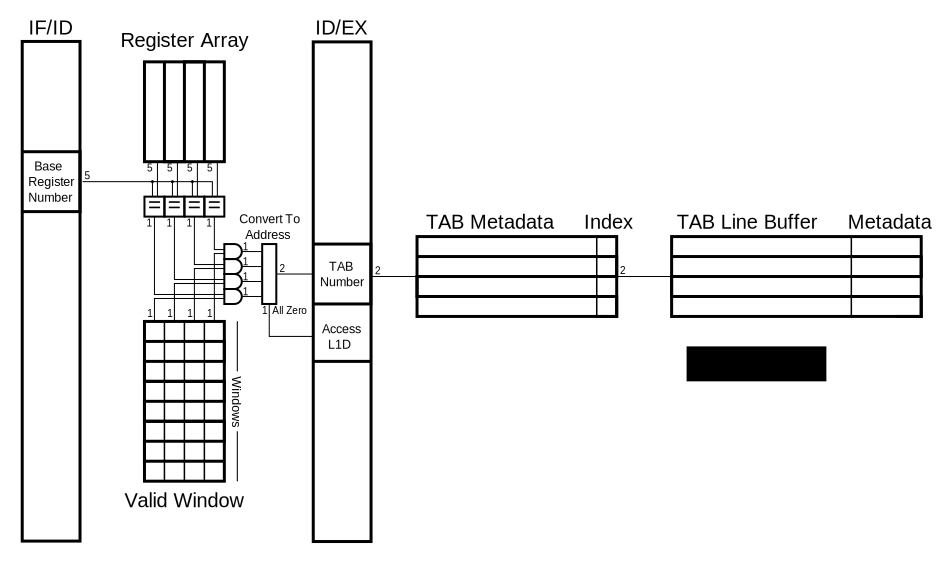
\includegraphics[width=\textwidth]{figures/tabhardware.pdf}
\end{frame}
\begin{frame}{TAB ID Stage}
   \begin{columns} %[c] for centered, [T] for top
      \column{.57\textwidth}
      \begin{block}{TAB Reference Detection}
         \begin{itemize}
            \item Compare memory reference's base register number against
               each TAB associated register number in parallel
            \item If any match AND the matching TAB is valid (\texttt{AND} bits 
               from comparison with current valid window), direct reference to TAB
            \item If none match, go the the L1D
         \end{itemize}
      \end{block}
      \column{.43\textwidth}
      \includegraphics[width=\textwidth]{figures/tabhardware_ID.pdf}
   \end{columns}
\end{frame}
\begin{frame}{TAB EX Stage}
   \begin{block}{TAB Metadata and Buffer}
      \begin{itemize}
         \item Separate metadata for TAB entry and TAB line
            \begin{itemize}
               \item Not necessarily a one-to-one relationship
                  between TAB entries and TAB lines
            \end{itemize}
         \item Line and line metadata are accessed through the index field 
            in the TAB entry
         \item Level of indirection between TAB entry and TAB lines allows
            multiple TABs to share the same line
      \end{itemize}
   \end{block}
   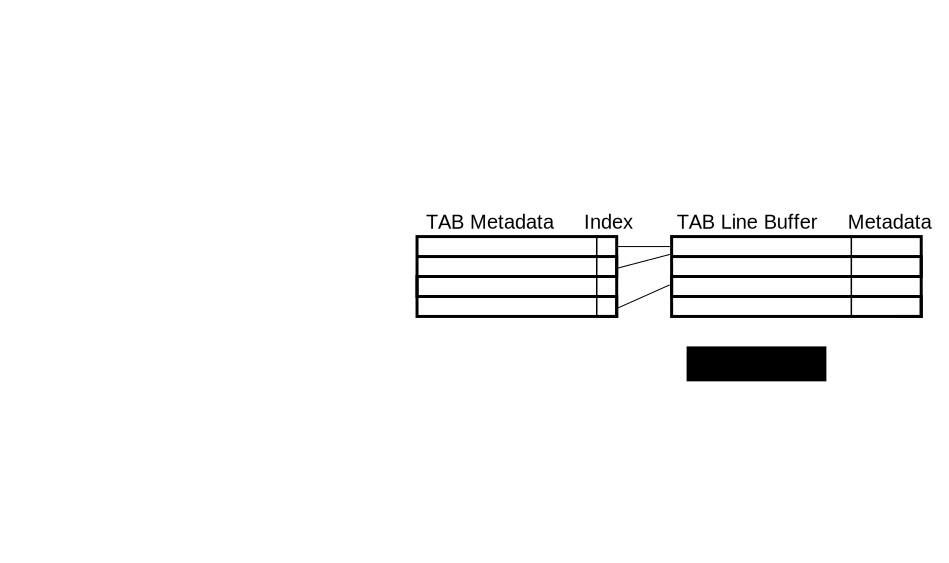
\includegraphics[width=\textwidth]{figures/tabhardware_EX.pdf}
\end{frame}
\begin{frame}{TAB Metadata}
   \begin{columns} %[c] for centered, [T] for top
      \column{.6\textwidth}
      \begin{block}{What is stored?}
         TAB metadata stores information about prefetching, the access type,
         and the TAB line it is using
         \begin{itemize}
            \item Access type helps save energy by stopping certain unnecessary 
               line transfers
            \item Stride, prefetch type and prefetch PC give information about how and
               when to prefetch
            \item Index and extra line indicate the TAB line(s) being used
         \end{itemize}
      \end{block}
      \column{.4\textwidth}
      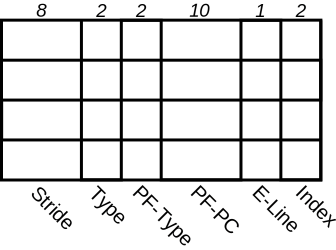
\includegraphics[width=\textwidth]{figures/tabmeta.pdf}
   \end{columns}
\end{frame}
\begin{frame}{Line Metadata}
   \begin{block}{What is stored?}
      Line metadata stores information which allows quick L1D access for
      writebacks and interferences
      \begin{itemize}
         \item Line number and way give exact L1D location of line
         \item Physical page number removes need to check the DTLB per access
         \item Write mask so only dirty bytes are written back to L1D
      \end{itemize}
   \end{block}
   \begin{center}
      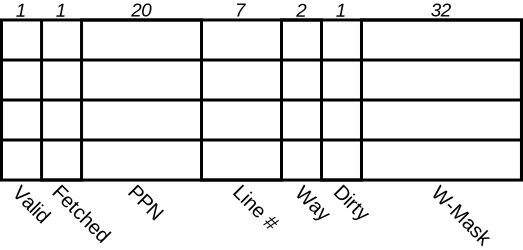
\includegraphics[width=0.55\textwidth]{figures/linemeta.pdf}
   \end{center}
\end{frame}
\subsection{Modifications Required for TAB}
\begin{frame}{ISA Modifications}
   \begin{block}{Extra instructions}
      \begin{itemize}
         \item Only requires one extra opcode: gtab and rtabs instructions
            are differentiated by a separate one-bit field
         \item Many fields in gtab are stored in metadata
            \begin{itemize}
               \item Base register stored in register array
               \item Stride is left shifted by value in shift size to give actual stride
               \item L/S is the prefetch type
               \item Prefetch offset multiplied by the instruction byte width is
                  added to the current PC to produce prefetch PC metadata field
            \end{itemize}
         \item rtabs release bitfield indicates TAB entries to deallocate
      \end{itemize}
   \end{block}
   \begin{center}
      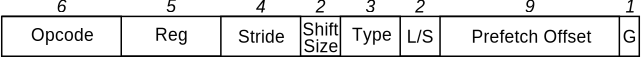
\includegraphics[width=0.85\textwidth]{figures/gtabformat.pdf}\\
      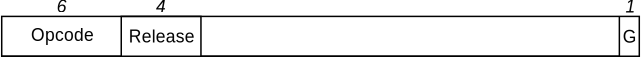
\includegraphics[width=0.85\textwidth]{figures/rtabformat.pdf}
   \end{center}
\end{frame}
\begin{frame}{Required L1D Changes}
   \begin{itemize}
      \item Each line in L1D is extended with two bits: the T and I bits
      \item T bit indicates if line resides in a TAB. L1D evictions use this bit
         to properly deallocate TAB line
      \item I bit indicates if references to this line should go to the TAB for
         the most recent data; this is called an "interference"
      \item Many lines that reside in the TAB are guaranteed not to cause interferences,
         hence the need for the separate I bit.
   \end{itemize}
\end{frame}
\section{TAB Operations}
\subsection{Basic TAB Functionality}
\begin{frame}{Allocation and Deallocation}
   \begin{itemize}
      \item gtab instruction allocates a TAB
         \begin{itemize}
            \item Deallocates existing TAB entry if still valid
            \item Updates register array to associate base register with TAB
            \item Prefetches first line to be accessed by TAB references
            \item Marks entry as valid
         \end{itemize}
      \item rtabs instruction deallocates one or more TABs
         \begin{itemize}
            \item Bitfield in rtabs states TABs to deallocate
            \item Only flush dirty bytes when deallocating
            \item Remove register association
         \end{itemize}
   \end{itemize}
\end{frame}
\subsection{Prefetch System}
\begin{frame}{Prefetching}
   \begin{block}{How prefetching works}
      \begin{itemize}
         \item TAB assumes it has the proper line at all times
         \item Can calculate the next TAB reference's address using stride information
         \item If next reference crosses line boundary, prefetch next line now
         \item Line is guaranteed (if valid), so no tag checks
         \item DTLB only accessed when prefetching first line or crossing
            a page boundary
      \end{itemize}
   \end{block}
   \begin{center}
      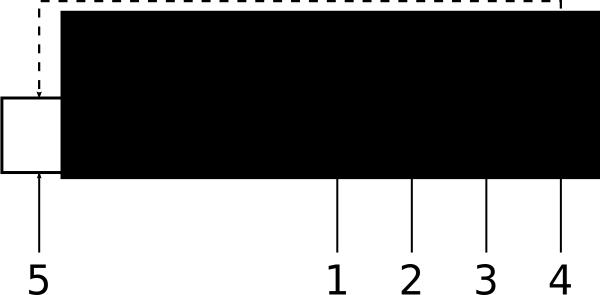
\includegraphics[width=0.45\textwidth]{figures/prefetch.pdf}
   \end{center}
\end{frame}
\begin{frame}{Prefetch Schemes}
   \begin{itemize}
      \item Not all TAB references should check for a prefetch
         \begin{itemize}
            \item Can't prefetch in conditionally executed code
            \item Shouldn't prefetch if future references use old line
            \item Some prefetch checks are wasteful
         \end{itemize}
      \item TAB references must fit into a prefetch scheme
         \begin{itemize}
            \item Can't indicate each and every prefetch individually through 
               just a gtab instruction
            \item Use a scheme instead to mark many instructions
            \item Either all loads, all stores, all loads and stores, or a single
               instruction causes a prefetch
            \item If single instruction prefetch, check current reference PC against
               stored PC
         \end{itemize}
      \item Only check for prefetch when indicated by the scheme
      \item If TAB references don't fit a scheme, can't allocate TAB
   \end{itemize}
\end{frame}
\subsection{Capturing More References}
\begin{frame}{Extra Line}
   \begin{itemize}
      \item Sometimes a TAB may require two lines instead of one
         \begin{itemize}
            \item TAB references may be accessed out of order, making 
               prefetching impossible
            \item Extra line solves this by letting us prefetch back and forth
               between two lines, keeping the line for references that need it
         \end{itemize}
      \item TAB references use the next high order bit after the line number
         to determine which TAB line to access
      \item Each line keeps track of prefetching and line metadata individually
      \item When an extra line is used, one less TAB entry can be allocated
   \end{itemize}
\end{frame}
\subsection{TAB and Function Calls}
\begin{frame}{Supporting Function Calls}
   \begin{itemize}
      \item Can't keep TAB across function calls
         \begin{itemize}
            \item Base registers used in caller loop may be reused for 
               different references in callee
         \end{itemize}
      \item Shouldn't just deallocate all TABs on a function call (inefficient)
      \item Use a window system to keep track of validity per call
         \begin{itemize}
            \item Each function call has its own set of TAB validity bits
            \item All TABs are marked invalid in new windows; other window
               validity kept intact
            \item A TAB is only valid in one window
            \item Allocating a TAB deallocates the TAB from previous windows
         \end{itemize}
   \end{itemize}
\end{frame}
\begin{frame}{Supporting Function Calls Example}
   \begin{block}{Pseudocode for valid windows}
      \begin{center}
         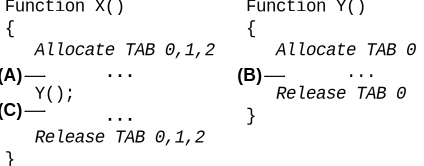
\includegraphics[width=0.65\textwidth]{figures/validexample1-1.pdf}
      \end{center}
   \end{block}
   \begin{block}{Valid windows at various points}
      \begin{center}
         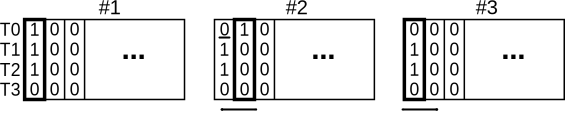
\includegraphics[width=0.85\textwidth]{figures/validexample1-2.pdf}
      \end{center}
   \end{block}
\end{frame}
\begin{frame}{Supporting Function Calls Continued}
   \begin{itemize}
      \item Since old TABs appear invalid on calls, references are directed to
         L1D appropriately
      \item All other TAB data is kept intact on function calls, 
         only validity is changed
      \item If function call does not use a TAB, it can stay valid for the caller
      \item If a caller TAB is reallocated in the callee, the caller can no longer
         use it when the callee returns
   \end{itemize}
\end{frame}
\section{Compilation}
\subsection{Compiler Analysis}
\begin{frame}{Compiler Requirements}
   \begin{itemize}
      \item No additional interprocedural analysis or code transformations
      \item Compiler must know TAB buffer line width and line count
      \item Compiler detects memory references with constant strides or with
         loop invariant addresses
      \item If references fit TAB constraints, compiler can generate a gtab in
         the loop preheader and an rtabs in the postheader
   \end{itemize}
\end{frame}
\begin{frame}{TAB Allocation Constraints}
   \begin{itemize}
      \item TAB references must all have the same base register
      \item No other references may use the TAB's base register
         while it is active
      \item TAB references must fit in a line and average more than 1 
         reference per line
      \item TAB references must fit one of the prefetch schemes and cannot require
         a prefetch in conditionally executed code
      \item TAB references must all be in the same loop
      \item Each TAB reference must have the same constant stride
      \item Maximum distance between any two TAB references is no more 
         than the line size
   \end{itemize}
\end{frame}
\begin{frame}{Allocation Heuristics}
   \begin{itemize}
      \item Can't allocate all potential TABs: in our case, we can have 
         four at one time
      \item Use a heuristic to select best energy saving TABs; ie the ones which
         may capture the most L1D references
      \item Rate each TAB reference based on estimated saved L1D accesses,
         then find the TABs with the most saved overall.
   \end{itemize}
\end{frame}
\begin{frame}{Allocation Heuristics Continued}
   \begin{itemize}
      \item Each reference starts with one saved L1D access
      \item References in conditionally executed code are halved
      \item References in inner loops are increased based on depth
      \item Add all TAB reference scores to get "estimated references" 
         saved for TAB per loop
      \item Subtract required L1D accesses per loop (both loads and stores)
         \begin{itemize}
            \item Prefetches require a load and store; frequency based on stride
         \end{itemize}
      \item Divide overall saved accesses by two if using an extra line
   \end{itemize}
   \begin{block}{TAB Score Equation}
      \begin{equation}
         (estim\_refs - (L1D\_loads + L1D\_writes)) / \#TAB\_lines
      \end{equation}
   \end{block}
\end{frame}
\begin{frame}{Allocation Heuristics Example}
   \begin{block}{Example Code}
      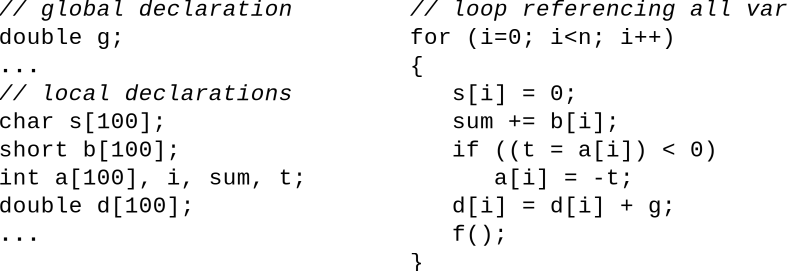
\includegraphics[width=0.65\textwidth]{figures/estimationexample_horizontal.pdf}
   \end{block}
   \begin{block}{Calculated Avoided L1D Accesses}
      \begin{center}
      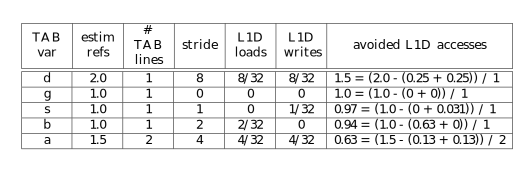
\includegraphics[width=0.80\textwidth]{figures/estimationtable.pdf}
      \end{center}
   \end{block}
\end{frame}
\begin{frame}{Avoiding Unnecessary Data Transfers}
   \begin{columns}
      \column{0.6\textwidth}
      \begin{block}{Read and Write Only TABs}
         \begin{itemize}
            \item Compiler controlled TAB means access patterns can be exploited to 
               further reduce energy
            \item Write maks can create a read-only TAB with no L1D writes
            \item TAB's "type" metadata field can indicate write first and write contiguous
               \begin{itemize}
                  \item \textbf{Write first:} TAB always writes bytes before reading.
                     Don't pull line from L1D
                  \item \textbf{Write contiguous:} All bytes in TAB line are written 
                     first. Don't pull line from L1D or L2D
               \end{itemize}
         \end{itemize}
      \end{block}
      \column{0.4\textwidth}
      \includegraphics[width=0.33\textwidth]{figures/memorytransfer_readonly.pdf}
      \includegraphics[width=0.33\textwidth]{figures/memorytransfer_writefirst.pdf}
      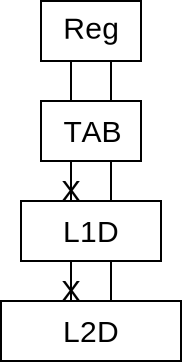
\includegraphics[width=0.33\textwidth]{figures/memorytransfer_writecontiguous.pdf}
   \end{columns}
\end{frame}
\section{Update Vs Original}
\subsection{Compare Update with Original}
\begin{frame}{Original Implementation}
   %\begin{block}{Original Implementation}
      \begin{itemize}
         \item Required bits from loads and stores to indicate TAB; used two opcodes
            \begin{itemize}
               \item Not backwards compatible
               \item Loads and stores lose part of their immediate field
            \end{itemize}
         \item Did not link base register to TAB
            \begin{itemize}
               \item TABs could have multiple registers
               \item TABs could stay active across function calls
            \end{itemize}
      \end{itemize}
   %\end{block}
   \end{frame}
      \begin{frame}{New Implementation}
   %\begin{block}{New Implementation}
      \begin{itemize}
         \item Does not require any ISA changes beyond one extra opcode
            \begin{itemize}
               \item Backwards compatible with existing code
               \item Easier to adopt
            \end{itemize}
         \item More strict and requires extra hardware due to base register association
            \begin{itemize}
               \item Captures less references due to strict requirements
               \item Higher chance to lose TABs on function calls
            \end{itemize}
      \end{itemize}
   %\end{block}
\end{frame}
\section{Results}
\subsection{Benchmarking}
\begin{frame}{How the TAB was tested}
   \begin{itemize}
      \item Use 20 benchmarks and large datasets from MiBench suite
      \item Compile benchmarks with VPO compiler
      \item Simulate in order five stage pipeline with SimpleScalar
      \item 32 byte L1D lines, 4 TAB lines, 16KB L1D
      \item Energy estimations from accurate 65nm CMOS library models
         using Synopsys Design Compiler
   \end{itemize}
\end{frame}
\begin{frame}{Testing Environment Details}
   \begin{block}{Energy Values}
      \begin{center}
         \vspace{-0.3cm}
         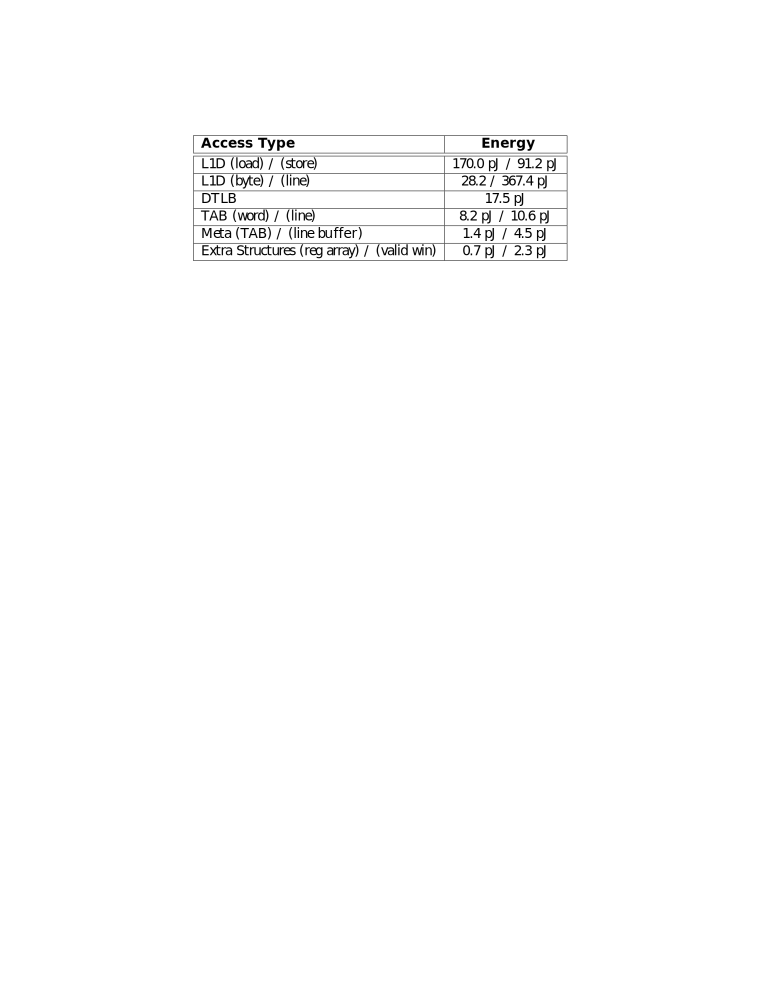
\includegraphics[scale=0.7]{figures/benchmarkenergy.pdf}
         \vspace{-0.3cm}
      \end{center}
   \end{block}
   \begin{block}{Benchmark Suite}
      \begin{center}
         \vspace{-0.3cm}
         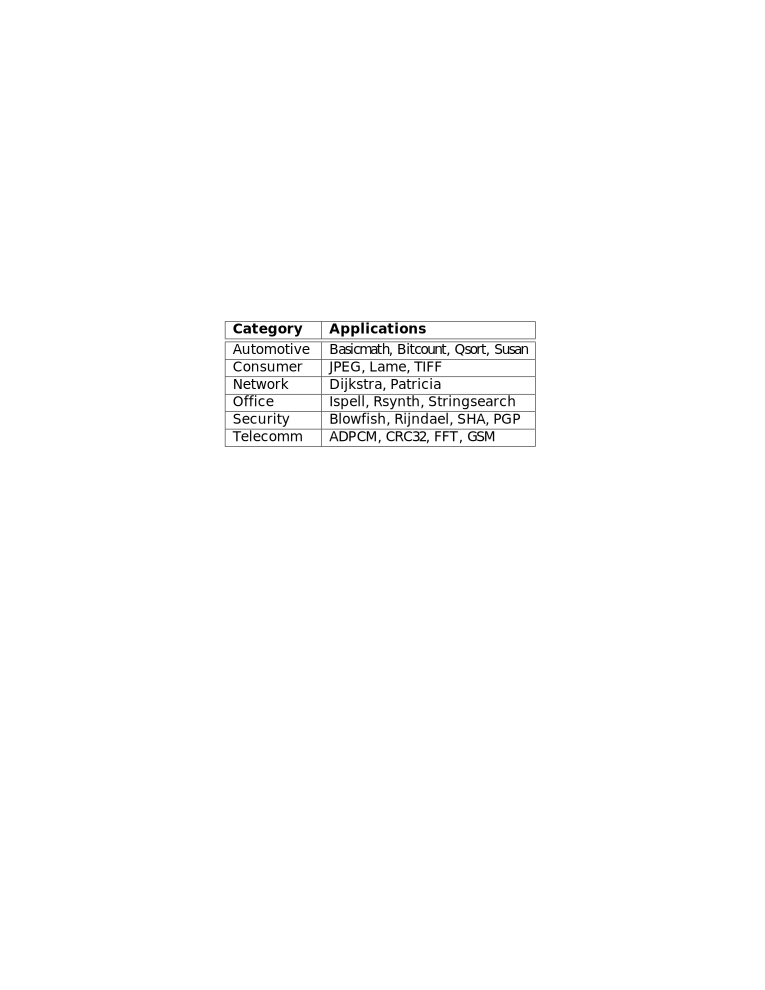
\includegraphics[scale=0.7]{figures/benchmarksuite.pdf}
         \vspace{-0.3cm}
      \end{center}
   \end{block}
\end{frame}
\subsection{Benchmark Results}
\begin{frame}{TAB Performance}
   With TAB enabled:
   \begin{itemize}
      \item \textbf{33.4\%} of all L1D references captured in TAB
      \item \textbf{30.9\%} fewer L1D accesses
      \item \textbf{1.7\%} less execution cycles
      \item \textbf{21.8\%} less energy used in L1D and DTLB
   \end{itemize}
\end{frame}
\begin{frame}{TAB Performance Graph: L1D Access Breakdown}
   \includegraphics[width=\textwidth]{figures/dl1_access.pdf}
\end{frame}
\begin{frame}{TAB Performance Graphs: Energy Breakdown}
   \includegraphics[width=\textwidth]{figures/energy_e_stage.pdf}
\end{frame}
\section{Conclusion}
\subsection{Final comparison}
\begin{frame}{TAB Update is give and take}
   \begin{itemize}
      \item Update requires far fewer ISA changes and is backwards compatible, but
         has reduced energy benefits
         \begin{itemize}
            \item Drop in TAB hits from 41.4\% to 33.4\%
            \item Increased execution time from 97.5\% to 98.3\%
            \item Decreased energy savings from 30.4\% to 21.8\%
         \end{itemize}
      \item Lower energy benefits almost entirely due to decreased TAB utilization
         caused by more strict TAB allocation requirements
   \end{itemize}
\end{frame}
\subsection{}
\begin{frame}{Conclusion}
   \begin{itemize}
      \item TAB reduces energy by capturing loop memory references in a small buffer
         which does not require tag checks and which greatly reduces DTLB accesses
      \item TAB updated to not require bits from loads and stores, making 
         it backwards compatible and easier to adopt
      \item Must sacrifice some energy savings for a less intrusive system
   \end{itemize}
\end{frame}
\end{document}
